\section{Tables \& Diagrams}
\subsection{Congestion Control FSM}
\begingroup
\renewcommand{\arraystretch}{1.5} % Default value: 1
\begin{center}
  \resizebox{8cm}{!}{
    \begin{tabular}{|l|l|l|}
      \hline
      \multicolumn{3}{|c|}{\Large{Slow Start}}                                                     \\
      \hline
      Event Trigger                & Transition to                  & Action(s)                    \\
      \hline
      \hline
      \multirow{3}{*}{new ACK}     & \multirow{3}{*}{loop back}     & cwnd $\to$ cwnd + MSS        \\
      ~                            & ~                              & dupACK $\to$ 0               \\
      ~                            & ~                              & transmit new segments        \\
      \hline
      dupe ACK                     & loop back                      & dupACK++                     \\
      \hline
      cwnd $\geq$ ssthresh         & Congestion Avoidance           & do nothing                   \\
      \hline
      \multirow{4}{*}{timeout}     & \multirow{4}{*}{loop back}     & ssthresh $\to$ cwnd / 2      \\
      ~                            & ~                              & cwnd $\to$ 1 MSS             \\
      ~                            & ~                              & dupACK $\to$ 0               \\
      ~                            & ~                              & re-transmit missing segments \\
      \hline
      \multirow{3}{*}{dupACK == 3} & \multirow{3}{*}{Fast Recovery} & ssthresh $\to$ cwnd / 2      \\
      ~                            & ~                              & cwnd $\to$ ssthresh + 3 MSS  \\
      ~                            & ~                              & re-transmit missing segments \\
      \hline
    \end{tabular}
  }
\end{center}%
\begin{center}
  \resizebox{8cm}{!}{
    \begin{tabular}{|l|l|l|}
      \hline
      \multicolumn{3}{|c|}{\Large{Congestion Avoidance}}                                                 \\
      \hline
      Event Trigger                & Transition to                  & Action(s)                          \\
      \hline
      \hline
      \multirow{3}{*}{new ACK}     & \multirow{3}{*}{loop back}     & cwnd $\to$ cwnd + MSS (MSS / cwnd) \\
      ~                            & ~                              & dupACK $\to$ 0                     \\
      ~                            & ~                              & transmit new segments              \\
      \hline
      dupe ACK                     & loop back                      & dupACK++                           \\
      \hline
      \multirow{4}{*}{timeout}     & \multirow{4}{*}{Slow Start}    & ssthresh $\to$ cwnd / 2            \\
      ~                            & ~                              & cwnd $\to$ 1 MSS                   \\
      ~                            & ~                              & dupACK $\to$ 0                     \\
      ~                            & ~                              & re-transmit missing segments       \\
      \hline
      \multirow{3}{*}{dupACK == 3} & \multirow{3}{*}{Fast Recovery} & ssthresh $\to$ cwnd / 2            \\
      ~                            & ~                              & cwnd $\to$ ssthresh + 3 MSS        \\
      ~                            & ~                              & re-transmit missing segments       \\
      \hline
    \end{tabular}
  }
\end{center}%
\begin{center}
  \resizebox{8cm}{!}{
    \begin{tabular}{|l|l|l|}
      \hline
      \multicolumn{3}{|c|}{\Large{Fast Recovery}}                                                      \\
      \hline
      Event Trigger             & Transition to                         & Action(s)                    \\
      \hline
      \hline
      \multirow{2}{*}{new ACK}  & \multirow{2}{*}{Congestion Avoidance} & cwnd $\to$ ssthresh          \\
      ~                         & ~                                     & dupACK $\to$ 0               \\
      \hline
      \multirow{2}{*}{dupe ACK} & \multirow{2}{*}{loop back}            & cwnd $\to$ cwnd + MSS        \\
      ~                         & ~                                     & transmit new segments        \\
      \hline
      \multirow{4}{*}{timeout}  & \multirow{4}{*}{Slow Start}           & ssthresh $\to$ cwnd / 2      \\
      ~                         & ~                                     & cwnd $\to$ 1 MSS             \\
      ~                         & ~                                     & dupACK $\to$ 0               \\
      ~                         & ~                                     & re-transmit missing segments \\
      \hline
    \end{tabular}
  }
\end{center}
\endgroup
\subsection{Delay (tabulation)} \label{ssec:delaytable}
\begin{center}
  \begin{tikzpicture}[
    scale = 0.75, transform shape,
    >={Latex[black, length=1mm]},
    node distance=2cm,
    roundnode/.style={
        circle, draw=black!80, fill=blue!5, minimum size=7mm
      },
  ]
  \node[roundnode](A) {A};
  \node[roundnode](R1) [right=of A] {R1};
  \node[roundnode](R2) [right=of R1] {R2};
  \node[roundnode](B) [right=of R2] {B};
  \node[node distance=0.25cm] [left=of A] {\qty{250}{\byte}};
  \path[-]
    (A) edge [] node[above]{\qty{8}{Mbps}} (R1)
    (R1) edge [] node[above]{\qty{2}{Mbps}} (R2)
    (R2) edge [] node[above]{\qty{8}{Mbps}} (B)
    (A) edge [] node[below]{\qty{2}{ms}} (R1)
    (R1) edge [] node[below]{\qty{4}{ms}} (R2)
    (R2) edge [] node[below]{\qty{2}{ms}} (B)
  ;
  \end{tikzpicture}
  \begin{scriptsize}
    \begin{itemize}
      \item sending 4 packets from A to B
      \item In diagram propagation dealay is below link, and speed is above.
      \item base output delay is the transmission delay $\frac{\ell_\text{\tiny{pkt}}}{S_\text{\tiny{link}}}$ (use same units)
      \item base input delay is just the propagation delay.
    \end{itemize}
  \end{scriptsize}
  \resizebox{8cm}{!}{
    \begin{tabular}{ |r|r|r|r|r|r|r| }
      \hline
      \multicolumn{1}{|c|}{\textbf{src}} & \multicolumn{1}{c|}{speed} & \multicolumn{1}{c|}{prop} & \multicolumn{1}{c|}{speed} & \multicolumn{1}{c|}{prop} & \multicolumn{1}{c|}{speed} & \multicolumn{1}{c|}{prop} \\
      \hline
      \textbf{base} & 0.25ms & 2.00ms & 1.00ms & 4.00ms & 0.25ms & 2.00ms \\
      \hline
      \hline
      \multicolumn{1}{|c|}{P$_{\#}$} & \multicolumn{1}{c|}{A$\to$} & \multicolumn{1}{c|}{$\to$R1} & \multicolumn{1}{c|}{R1$\to$} & \multicolumn{1}{c|}{$\to$R2} & \multicolumn{1}{c|}{R2$\to$} & \multicolumn{1}{c|}{$\to$B} \\ [0.6ex]
      \hline
      1 & 0.25ms & 2.25ms & 3.25ms & 7.25ms & 7.50ms & 9.50ms \\
      \hline
      2 & 0.50ms & 2.50ms & 4.25ms & 8.25ms & 8.50ms & 10.50ms \\
      \hline
      3 & 0.75ms & 2.75ms & 5.25ms & 9.25ms & 9.50ms & 11.50ms \\
      \hline
      4 & 1.00ms & 3.00ms & 6.25ms & 10.25ms & 10.50ms & 12.50ms \\
      \hline
    \end{tabular}
  }
\end{center}
\begin{scriptsize}
  First fill the entire table using the base delay for each column. Now
  modify the table left to right and top to bottom without skipping
  columns. For every output column ($X\to$) take each term and add to it
  the max of the term to the left and above (use 0 if there is none).
  Then for every input column ($\to X$) simply add to each term the
  value of the column to the left.
\end{scriptsize}
\subsection{The Big Picture}
\begin{center}
  \resizebox{8cm}{!}{
  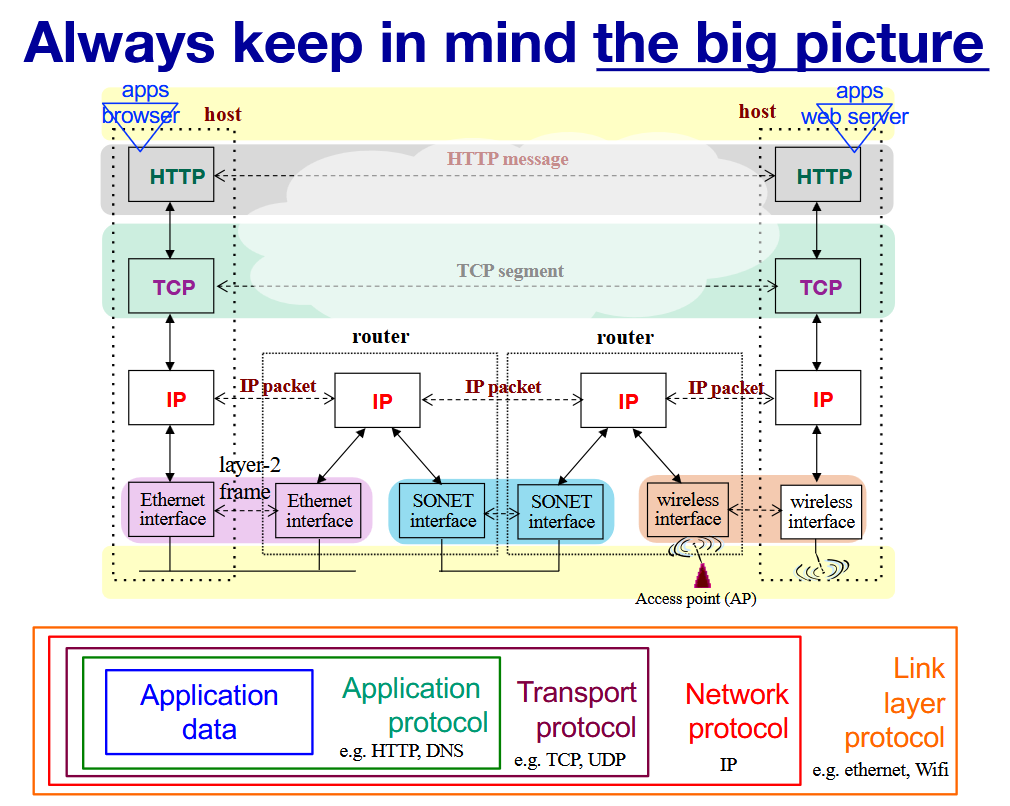
\includegraphics[]{images/big-picture.png}
  }
\end{center}